\documentclass[a4paper, 11pt,titlepage]{article}
\usepackage[english]{babel}
\usepackage{amsthm, amsmath, amssymb}
\usepackage{graphicx}% includegraphics
\usepackage{array}   % outline of p{} elements in tables
\usepackage{enumitem}% control spacing in lists
\usepackage{caption} % for non-floating tables
\usepackage{subcaption} % for subfigures
\usepackage{listings}
\usepackage{enumitem}

\usepackage{fancyhdr}
\pagestyle{fancy}
\rhead{\leftmark}
\lhead{}
\lfoot{CONCEPT \today}
\rfoot{\thepage}
\cfoot{}

\lstset{numbers=left,
language=C
}

\usepackage[
  pdfborder={0,0,0},
  colorlinks=true,
  linkcolor=black,
  citecolor=black,
  urlcolor=blue
]{hyperref}
\usepackage{natbib}
\bibliographystyle{chicago}

\newtheorem{demand}{Demand}
\newtheorem{definition}{Definition}
\newtheorem{theorem}{Theorem}
\newtheorem{example}{Example}


\renewcommand{\familydefault}{\sfdefault}

\newcommand{\code}[1]{\texttt{#1}}
\newcommand{\waar}{{\normalfont \texttt{True}}}
\newcommand{\onwaar}{{\normalfont \texttt{False}}}
\newcommand{\na}{{\normalfont \texttt{NA}}}

\newcommand{\la}[1]{\boldsymbol{#1}}

\title{Validation report structure}
\author{Mark van der Loo and Olav ten Bosch\thanks{
Statistics Netherlands, Henri Faasdreef 312 2492 JP The Hague
}}
\date{\today\\
\vspace{1cm}
Deliverable xx for the ESSnet Validat Integration
}

\newenvironment{spec}[2]
{
\begin{minipage}{\textwidth}
\begin{center}
\captionof{table}{#1. Fields marked with a ${}^\dagger$ are for
validation results only. The number of fields is #2extendable. }
\begin{tabular}{|p{0.11\textwidth}p{0.11\textwidth}p{0.325\textwidth}p{0.325\textwidth}|}
\hline
\textbf{Item} & \textbf{Format} &\textbf{Description} &\textbf{Example}\\
\hline
}
{
\hline
\end{tabular}
\end{center}
\end{minipage}
}
\setlength{\parindent}{0pt}
\setlength{\parskip}{2ex}

%%%%%%%%%%%%%%%%%%%%%%%%%%%%%%%%%%%%%%%%%%%%%%%%%%%%%%%%%%%%%%%%%%%%%%%%%%%%%%%
\begin{document}

\maketitle{}

\tableofcontents{}

\newpage

\section{Introduction}
\label{sect:introduction}

Data validation is at the core of every production chain in official statistics.
Whether it is the input received via a survey, a bunch of data records transferred from an administrative source or a register or the result from some internet scraping,
data must be checked against its expectations to process it and finally publish it.
For a more detailed explanation of data validation in general and the principles we identified in validation, we refer to the 
handbook of data validation [ref] and the appendix of the Business architecture on validation [ref].

Standardisation is important in official statistics and this also applies to validation processes.
Especially in the case of cross-organisation validation, where both a data producer and a data receiver check the same data against some
commonly agreed validation rules, standardisation is crucial to prevent different interpretations of the results.
The more harmonised validation reports are, the better the understanding across organisations is.
This has been recognized by the ESSnet on Validation project (Validat Integration) and thus a Work Package (WP2) was added to attack this issue.
This report is one of the deliverables of Work Packages 2.
It contains the result of the work carried out by various project partners and focusses on the standardisation of the output of a validation process: the \emph{validation report}.

Obviously we are interested in the question what information can and should be included in a validation report and the optimal way to express this information.
In this document we develop a \emph{generic} structure for expressing validation results.
We have the ambition to develop a validation report structure that can be used in \emph{any validation task} in \emph{any organisation} in any \emph{statistical domain}. 
To make it applicable in machine to machine communication contexts as well as in human contexts we design a machine-readable as well as a human readable format.

The approach we have taken is a combination of a top-down apprach and a botom-up approach.
In the bottom-up approach a number of example validation reports from member states and Eurostat were collected and studied to identify common elements.
This resulted in a long-list of validation report elements categorized into several classes such as rule metadata, process metadata, aggregates etc.
This led to some thinking about the basic concepts that are used in validation reports across the ESS.
We used the results from the bottom-up approach to develop a more formal top-down approach expressed in this report.
Step by step we built a validation report structure that is generic enough to be used in a wide range of validation contexts in many institutes,
expressive enough to support the most recognized validation report elements recognized from the bottom-up approach and
flexible enough to be adapted in a regional validation context while containing the standardized elements from the generic format.
Validation tools or other statistical tools producing validation reports as a side product should be able to use this structure for its validation output.

In this deliverable we address the following aspects:
In chapter 2 we ask ourselves what we should expect from a generic validation report structure.
After some elaboration on the variety in richness of a validation report, we define a number of generic demands.
In chapter 3 we define some core elements to be used in the definition of the validation report structure such as a validation result and a validation event.
In chapter 4 we formally define a validation report and propose a JSON-concept scheme for a basic machine-readable validation report.
This basic scheme leaves out aggregation facilities, which complicates the design considerably.
We describe the possibilities to add aggregation facilities to the report structure in chapter 5 and propose a JSON-concpet scheme for such message as well.
Chapter 6 shows some examples of validtaion reports, expressed in the schemes derived in chapters 4 and 5.
chapter 7 explains how a machine readable format can be transformed into a human readable format.
Chapter 8 presents a brief conclusion.




\section{Demands on a validation report}
\label{sect:demands}
Figure~\ref{fig:validation} gives a high-level overview of a data validation
procedure. At the input side, we find the data to be validated and the
validation rules that the data are supposed to satisfy. At some point in time,
the data are confronted with the rules and validation results are created. 
%
\begin{figure}[t]
\centering
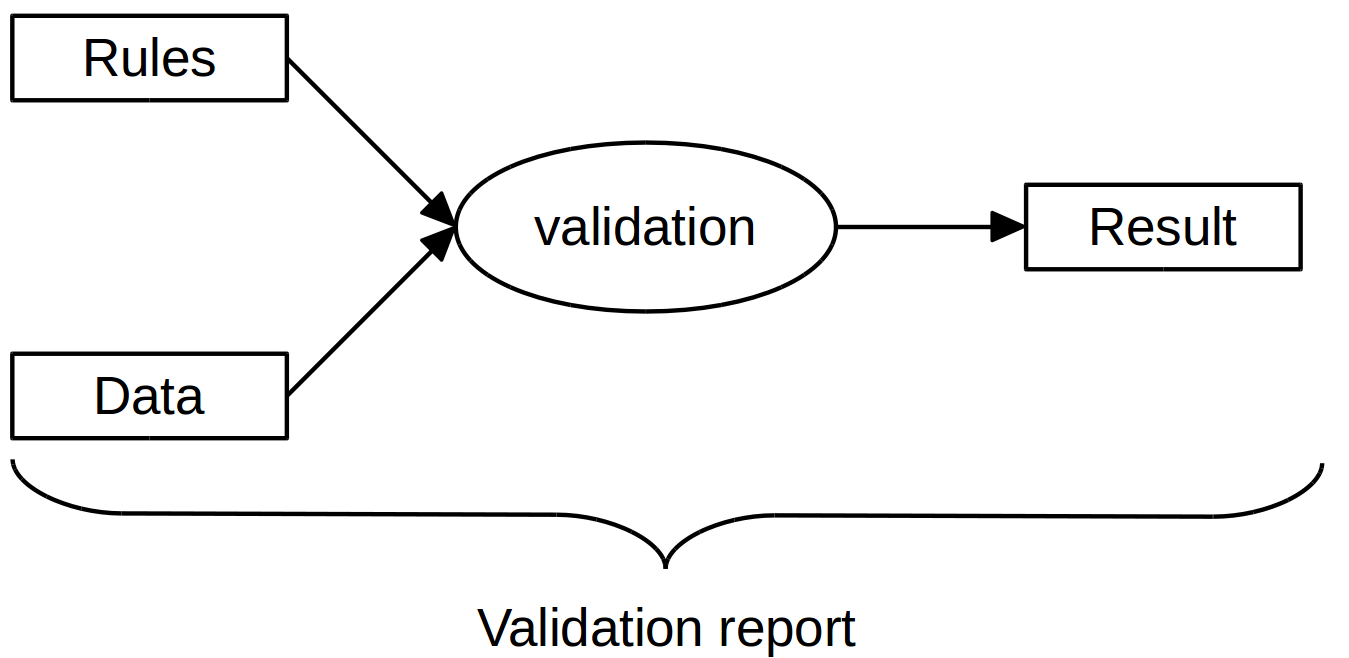
\includegraphics[width=0.7\textwidth]{fig/validation.png}
\caption{Information elements involved in creating a validation result, relevant for validation reports.}
\label{fig:validation}
\end{figure}

The purpose of a validation report is to convey validation results and
information on the validation procedure. The procedure as a whole generates and
processes a lot of information that can possibly be included in such a report.
For example, the validation rules may be endowed with metadata such as
descriptions and severity level and for the validation procedure it may be
interesting to record a timestamp and the used software.

A relevant question to ask is therefore what information should be included in
a validation report. Conceptually we can explore the extreme possibilities on a
scale such as depicted in Figure~\ref{fig:richness}. On the left, we find a minimal report
containing a single result only: True, meaning that all data passed all rules,
or False, meaning that not all data passed all rules. On the right extreme, the
report conveys all data and metadata associated with the validated data, the
validation rules, the validation procedure and the results.
%
\begin{figure}
\centering
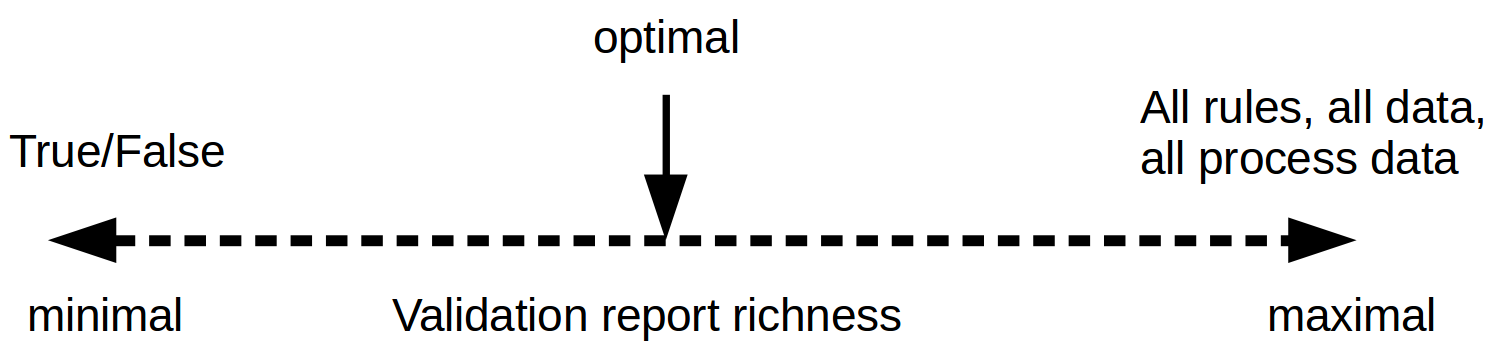
\includegraphics[width=0.8\textwidth]{fig/richness.png}
\caption{Possible content of validation reports on a conceptual scale of 'richness'.}
\label{fig:richness}
\end{figure}


Before moving to a formal discussion of the information items involved with
data validation, it is useful to discuss a number of demands on a validation
report that will serve all uses and users. First of all, we take as a given
that a result that cannot be identified with the data and rules it pertains to
is useless. If the reports are to be used for communication accross
organizations, or if they are to interpreted separately from the process that
triggered the validation, the relation with the rules and data needs to be
included.  In fact, this can also be seen as a direct consequence of the
validation principle \emph{Well-documented and appropriately communicated
validation errors} \citep{ESS2017}. This leads us to the following demand.

\begin{demand}[Identification]
A validation report shall convey validation results such that they can be
identified with the validation procedure, the validation rules used, and the
validated data.
\label{dem:identify}
\end{demand}


A validation procedure usually involves multiple rules and each rule may
pertain to different subsets of variables, records or reference datasets. Every
confrontation of a rule with the data can be seen as a validation
(sub)procedure yielding a validation report. To gather all results, validation
reports should be able to be combined to an overall report.
%
\begin{demand}[Closure under combination]
Two validation reports shall be combinable in such a way that the result is
again a validation report that includes all information that separate reports
contained.
\label{dem:combine}
\end{demand}
%
This includes cases where multiple procedures are involved, possibly pertaining
to varying datasets, rulesets and actors involved in the validation procedures. 

Finally, depending on intended use, one may be interested in the details of
each step in each validation procedure, or in a more aggregated view of one or
more validation events. Indeed, a quick view on some example validation reports
from multiple NSI's and multiple statistical domains shows that most of them
contain some kind of aggregated results within the validation report itself.
Therefore, we also demand the following.

\begin{demand}[Closure under aggregation]
A validation report can be aggregated such that the result is again a
validation report.
\label{dem:aggregate}
\end{demand}

Here, many types of aggregation may be relevant, including counting the
(relative) number of passes and fails, finding the procedure that yielded the
maximum number of fails (or passes), and so on.

Both the second and third demand mention the term \emph{closure} which may not be a
familiar term to all readers. The term `closure' or `algebraic closure' refers
to the property of a set being invariant under certain operations. For example,
becayse the sum of any two natural numbers is again a natural number, we can say
that ‘the natural numbers are closed under addition’. For our purposes it is
important that the result of combining or aggregating a validation report is
also a validation report, meaning that it has exactly the same structure (but
possibly different content) before or after aggregation. If this is not the
case, we run the risk of defining new data structures for each aggregate or
combination of reports.

As it turns out, adding both closure under combination and closure under
aggregation to the demand of identifiability significantly increases the
complexity of the structure of a validation report. Since aggregates can always
be derived from a set of `atomic' validation results, we therefore propose two
types of interchange formats. The first is called the \emph{basic validation
report structure} and it conveys the rule-by-rule and event-by-event validation
results, dropping Demand~\ref{dem:aggregate}. It is a simple format that is
representable as a rectangular data structure from which (possibly grouped)
aggregations can easily be computed.  The second is called \emph{extended
validation report structure}. This structure is richer and allows for
precomputed aggregates.  Since aggregation imposes a graph structure on a
record set, parsing such a structure is more involved.





\section{Evaluation events}
\label{sect:evaluations}
Figure~\ref{fig:eval} depicts the concepts involved in creating a result by
evaluating a validating or aggregating expression. Conceptually, the \textsf{data}
consists of values bound to variable names. The \emph{expression} denotes, using
a fixed set of syntax rules, a computation on variables present in the \emph{data}.
In the \emph{evaluation} event, the following activities take place
\begin{enumerate}[noitemsep]
\item Read the expression and check whether it is valid syntax. If not: stop execution.
\item Parse the expression: substitute variable names with the corresponding values
stored in \emph{data}.
\item Evaluate the expression, creating the \emph{result}.
\end{enumerate}
In actual implementations these processes can be optimized. For example when
the same expression is evaluated with multiple data sets, the first step needs
to be executed only once. As a demonstration that both validation and
aggregation fit in this description, consider the following two examples.
%
\begin{figure}
\centering
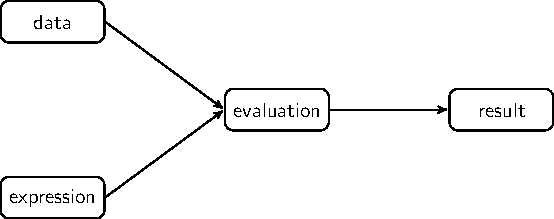
\includegraphics[width=0.8\textwidth]{fig/eval.pdf}
\caption{Concepts involved in evaluating a (validating or aggregating) expression.}
\label{fig:eval}
\end{figure}

\begin{example}
Consider the expression
\begin{align*}
\texttt{age >= 0}
\end{align*}
and a data record given by
\begin{center}
\begin{tabular}{lll}
Name & Age & Sex \\
\hline
Joe  & 17  & male
\end{tabular}
\end{center}
In the first step, the evaluator reads in the expression and approves it after
checking with the syntax. In the second step, the variable names are identified
and replaced with matching values from the dataset. This yields \code{17 >= 0}.
Finally, in the third step the proposition \code{17 >= 0} is evaluated and the
result returned.
\end{example}

\begin{example} Consider the following table of validation results (we use
1 for \waar{} and 0 for \onwaar{}).
\begin{center}
\begin{tabular}{lr}
Name  & validation\_result \\
\hline
Alice & 1    \\
Bob   & 1    \\
Carol & 0    \\
\end{tabular}
\end{center}
The expression counting the number of passes is given by
\begin{align*}
\texttt{sum(validation\_result)}.
\end{align*}
In the first step the evaluator reads in the expression and approves it after
checking with the syntax. In the second step, the variable names are identified
and the expression is expanded\footnote{Conceptually of course. In practice
accumulation will be more efficient.} to \code{1 + 1 + 0}.  This expression is
then evaluated and its result returned.
\end{example}
Obviously, to  interpret a result, both the input data and the
expression used must be known. However, the value of the final result may also
depend on the (version of) the evaluator. Especially since the Handbook on
Validation explicitly includes the possibility of validation being done by
expert review. In that case, the `expression' may be a manual or handbook with
recommendations on evaluating a certain dataset and the result is a validity
assessment by an expert. But even in the case of formalized expressions,
interpreters may differ. Formal programming syntax standards often leave
certain details to interpreter developers. This inevitably leads to
platform-dependent results. 

It is therefore proposed here to include metadata elements that identify data,
expression, and the evaluating event for all results reported in a validation
report, whether they are aggregates or validation results. Since validation
results have a particular type and meaning that differs from aggregation
results it will be useful to differentiate their metadata as well.











%%%%%%%%%%%%%%%%%%%%%%%%%%%%%%%%%%%%%%%%%%%%%%%%%%%%%%%%%%%%%%%%%%%%%%%%%%%%%%%
\section{Identifying validation results}
\label{sect:identifying}
To get an idea of the (meta)data necessary to identify a validation result,
consider the data, validation rules and validation results shown in
Table~\ref{tab:example1}. When a dataset is confronted with a validation rule,
there are three possible outcomes. A rule can be satisfied, yielding \waar{}, a
rule can be failed, yielding \onwaar{}, or a rule cannot be evaluated because
of missing data, yielding \na{}.
%
\begin{table}
\centering
\caption{Example data, validation rules, and results}
\begin{tabular}{rccccb{4cm}}
\hline
&\multicolumn{2}{c}{\textbf{Variables}}&&\multicolumn{2}{c}{\textbf{Rules}}\\
Nr  & Age  & hasjob     && \code{Age >= 0} & \code{IF Age < 15 THEN hasjob == `no'}\\
\cline{2-3}\cline{5-6}
1   & 36   & \code{yes} && \waar{}        & \multicolumn{1}{c}{\waar{}}\\
2   & 53   & \code{NA}  && \waar{}        & \multicolumn{1}{c}{\na{}}\\
3   & 11   & \code{yes} && \waar{}        & \multicolumn{1}{c}{\onwaar{}}\\
\hline
\end{tabular}
\label{tab:example1}
\end{table}



In the example three records on age and work status are checked against two
rules: age must be larger than or equal to zero, and persons under 15 years old
cannot have a job. In each case the demand on  age can be checked and and each
record passes this test, yielding \waar{} as validation result. For the second
rule, the first record passes the check since age equals 36 and the person has
a job which is allowed by the rule. In the second case the job status is not
available (\na{}). Hence the rule cannot be checked and the returned value is \na{}
as well. Finally, in the third record there is an 11-year old with a job which
is a combination that is not allowed by the rule, yielding \onwaar{}.


The above discussion leads to the following definition of a validation result.
%
\begin{definition}[Validation result]
A validation result is a value from the set $\{0,1,\na{}\}$.
\label{def:validationresult}
\end{definition}
Validation results are obtained as outcomes of evaluating a validation rule on
a data set. We also follow the common convention which identifies $0$ with
\onwaar{} and $1$ with \waar{}.  The numeric representation will make it easier
to define aggregators in later chapters. 


A recurring point of discussion is whether \na{} should be an allowed
validation result. The main other options are to either interrupt execution, or
to interpret the result as failed (\onwaar{}) when one of the data points
necessary for evaluating a rule is missing. Because statistical data often
suffers from missing data the first option would yield many interruptions of a
statistical process flow, unless each rule guards against it by building in
clauses that detect missing values explicitly. The second option (\na{} implies
\onwaar{}) would yield a loss of information. More importantly, it assumes
(possibly unwarranted) that the user of the result follows this interpretation.

We deem both alternatives undesirable and therefore follow the definition
above, which also agrees with the definition of a formal data validation
function in the Methodology on Validation handbook published by the Validat
Foundation ESSnet \citep{zio2015methodology}.



With a \emph{validation event} we mean the physical activity where a dataset is
confronted with a single rule, yielding precisely one validation result. A
validation event is characterized by its inputs (the rule and the dataset it
pertains to) as well as its own metadata, including the time of execution and
the actor performing the execution. We adopt the following convention for
pairing the result of such an event with its identifying metadata.
%
\begin{definition}[confrontation] 
A \emph{confrontation} is a tuple $(e,r,d,v)$, where $e$ identifies the physical
validation event, $r$ identifies the evaluated validation rule, $d$
identifies the data points involved in the evaluation and $v$ is the
generated validation result.
\label{def:confrontation}
\end{definition}
%
We leave open the possibility that the components $e$, $r$ and $d$ consist of
informative tuples to identify subcomponents of the event, data or rule. Note
that the above `definition' is not a definition in the mathematical sense.
Rather it is a convention that can be tested in a (software) environment where
data, rules, and validation events have been labeled and stored.




\section{Aggregation}
In the context of validation, commonly reported aggregates include the total
number or fraction of rules violated or the number or fraction of records  that
violate a certain rule. The latter aggregates may be reported for the whole
population or for each relevant subpopulation (e.g. by economic activity for a
business survey). 


Before discussing how we endow machine-readable validation reports with
identifiable and combinable aggregates, it is useful to point out some of the
subtleties that arise when thinking of aggregation in a general way. The first
subtlety has to do with counting rules and counting validation results.
Consider as an example the rules \code{turnover >= 0} and \code{mean(profit) >=
0}.  When applied to a set of $n$ business records containing the variables
\code{turnover} and \code{profit}, the first rule is evaluated $n$ times in $n$
validation events, yielding $n$ validation results. The second rule is
evaluated in a single validation event, yielding a single validation result,
regardless of the number of records in the dataset. This means that an
aggregate such as `the total number of rules violated' is ill-defined. It is
only meaningful to talk about `the number of events that resulted in
\onwaar{}'. 

The second subtlety is that a set of aggregates can again be combined to form
new aggregates. For example, in a first step we may compute the fraction of
events yielding \onwaar{} per economic sector. In a next step we count for how
many sectors this number is less than or equal to 0.05.

Figure~\ref{fig:graphs} illustrates the above points in a graph-like structure.
Suppose we start with a basic report containing five validation results. We can
add an aggregate counting the number of passes in a certain subset
(Figure~\ref{fig:graph1}).  In Figure~\ref{fig:graph2}, a second count is
added, as well as an overall count that is composed of the two low-level
aggregates. Figure~\ref{fig:graph3} depicts a situation where a subset of
validation results are combined to form aggregates of several types: the number
of passes and the fraction of passes.
%
\begin{figure}[!t]
  \centering
  \begin{subfigure}[b]{0.7\textwidth}
    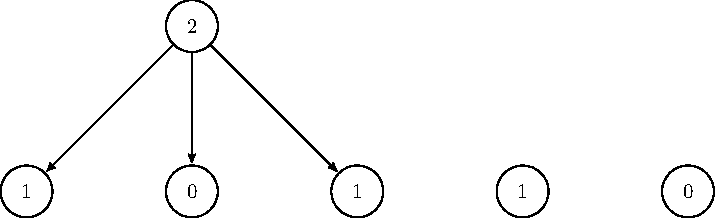
\includegraphics[width=\textwidth]{fig/graph1.pdf}
    \caption{Validation report with a single aggregated value.}
    \label{fig:graph1}
  \end{subfigure}
  \begin{subfigure}[b]{0.7\textwidth}
    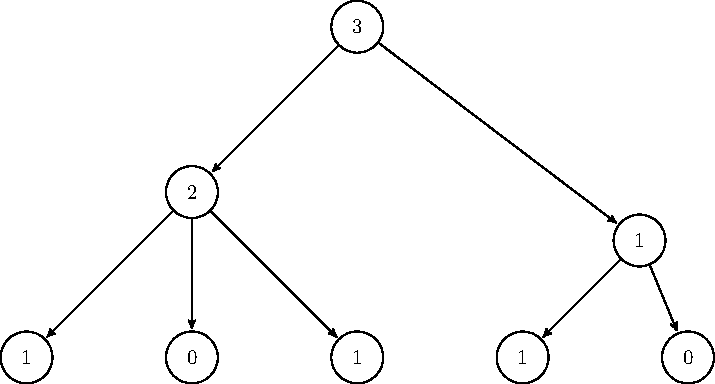
\includegraphics[width=\textwidth]{fig/graph2.pdf}
    \caption{Validation report with multiple aggregates.}
    \label{fig:graph2}
  \end{subfigure}
  \begin{subfigure}[b]{0.7\textwidth}
    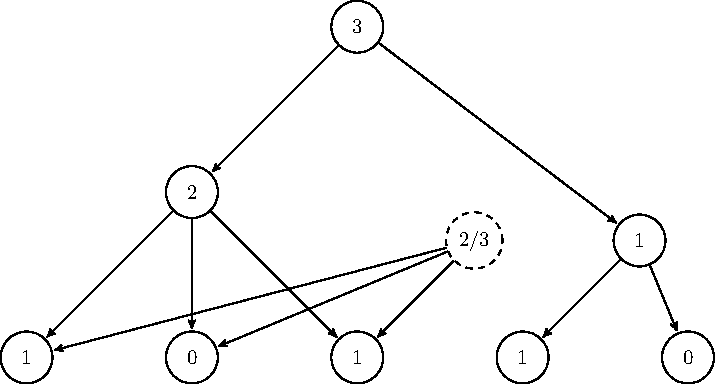
\includegraphics[width=\textwidth]{fig/graph3.pdf}
    \caption{Validation report with aggregates of various types.}
    \label{fig:graph3}
  \end{subfigure}
  \caption{Structure of validation reports including aggregates, of varying complexity.}
  \label{fig:graphs}
\end{figure}

These examples suggest that aggregates can be interpreted as nodes in a
directed graph where the edges (arrows) point from the aggregate to the nodes
used to compute the contents of the node. Nodes that have no outgoing edges
(leaves) correspond one-to-one with validation results.  The collection of
nodes and edges contain sufficient structure to make the representation of
validation reports identifiable, combinable, and (recursively) aggregable. In
the following paragraph we define more closely the type of graph that can be
used to represent an aggregation structure.


%%%%%%%%%%%%%%%%%%%%%%%%%%%%%%%%%%%%%%%%%%%%%%%%%%%%%%%%%%%%%%%%%%%%%%%%%%%%%%%
\subsection{Aggregation graphs}
\label{sect:aggregationgraphs}
Graphs are well-known mathematical structures that represent connectivity
between objects. Indeed, the  study of graphs dates back to the 18th century
when Leonhard \citet{euler1741solutio} solved the famous K\"oningsberger
bridges problem.  For our purposes, a graph will serve as a model to store
validation results, aggregates thereof, and the operations that lead to the
aggregated values.

The need for a graph structure rather then a more simple record-like structure
arises from the demand that reports be combinable to a new report.  To see
this, consider the following example. Two institutes validate a dataset with
turnover values against the rule \code{turnover >= 0}. The first institute
reports the fraction of passes, while the second institute reports the results
for each individual record. If these reports were naively combined, one could
misinterpret the fractional value reported by the first institute as pertaining
to the separate values reported by the second institute. A second example
occurs when the first institute creates a report containing both the individual
results and the aggregated fraction of passes. If this report is to be
augmented with new information, for example when new records come in it should
be clear from the report that the reported fraction of passes does not pertain
to the records added later.


Graphs basically consist of elements of some set, called \emph{nodes} or
\emph{vertices} and connections between them, which are called \emph{edges} or
\emph{arrows} if they are directed. Structured information can be stored by
endowing the nodes and edges with parcels of data.  Depending on the type and
number of edges allowed between the nodes, graphs are classified in a broad
number of types.  Below we define simple directed graph that comes close to our
purpose of structuring validation aggregates.
%
\begin{definition}
\label{def:simplegraph}
A \emph{simple finite directed graph} is a pair  $(V,E)$ where $V$ is a finite set and $E$
is a set of pairs $(v_1,v_2)$ with $v_1,v_2\in V$ and $v_1\not=v_2$.
\end{definition}
In this definition, the term \emph{simple} means that there are no loops (edges
that start where they begin, like $(v_1,v_1)$). The term \emph{directed} mean
that edges have a direction: the edge $(v_1,v_2)$ can be thought of as an
arrow, pointing from $v_1$ to $v_2$ and therefore differs from ($v_2$,$v_1$).
The term \emph{simple} also indicates that each pair of nodes is connected by
at most two, opposite pointing arrows.

A validation report can be represented by a more special graph. To define
it, we first need the concept of a path.
\begin{definition}[path, cycle]
\label{def:pathcycle}
Given a simple finite directed graph $(V,E)$. A \emph{path} is a sequence of
edges $e_1,e_2,\ldots,e_n$ such that the start of $e_j$ is equal to the end of
$e_{j+1}$ for $j=2,3,\ldots,n$. A \emph{cycle} is a path such that the end of
$e_n$ is equal to the start of $e_1$.
\end{definition}
A path is thus a sequence of connected edges. Since aggregation works bottom-up
and not top-down, we define the following graph to represent an extended
validation report.
\begin{definition}
A \emph{directed acyclic graph} is a simple finite directed graph $(V,E)$ with
the condition that $E$ contains no cycles.
\end{definition}
%
The term `directed acyclic graph' is often shortened to DAG in literature. This
particular structure has many technical applications, For example, the DAG
stands model for data processing flow in the SPARK model for distributed
computing \citep{gupta2003spark}. 


Simple graphs have a natural rule of composition. The `sum' of two simple
(directed) graphs is obtained as the union of the two vertex sets and the union
of the two edge sets. For a DAG, this combination rule does not always apply
since we are not allowed to have more than a single edge between any pair of
nodes.  We therefore define the following compatibility rule for directed acyclic
graphs.
\begin{definition}[Compatible DAGs]
\label{def:compatibledag}
Given two DAGs $G=(V,E)$ and $F=(V',E')$. These graphs are called
\emph{compatible} when the combination
\begin{align*}
G\oplus F = (V\cup V', E\cup E'),
\end{align*}
is also a DAG.
\end{definition}
Any software that combines extended validation reports (validation reports
including aggregates, to be defined below) should therefore always check for
compatibility of the reports upon combination.

\subsection{Identifying aggregates}
To understand the meaning of an aggregate value, one needs to identify the data
used to construct it (other nodes in the DAG of which the aggregate is a
member) as well as the way it was constructed. We therefore propose the
following definition.

\begin{definition}[aggregation]
\label{def:aggregation}
An \emph{aggregation} is a triple $(f,s,x)$ where $f$ identifies the function
used for aggregation, $s$ identifies the set of nodes used for aggregation and
$x=f(s)$ is the aggregate.
\end{definition}
Just like Definition~\ref{def:confrontation}, this is not a definition in a
precise mathematical sense. Rather it is something that can be tested in a
particular practical software/data environment. 

Also observe that we have not specified a codomain (range) for the aggregating
function $f$. We keep the definition general by design since aggregating
functions can have several relevant output types, some examples:
\begin{itemize}
\item the number of events resulting int \waar{} (numeric);
\item the rule that is violated most often (a string identifying the rule);
\item whether all events resulted in \waar{} (validation result).
\end{itemize}
The only thing that is important for a aggregating function is that it results
in a single value, in the sense that the result pertains to the whole subset
$s$ on which $f$ acts.



\section{Validation reports}
\label{sect:basicreports}
Recall that a \emph{validation} is a tuple $(e,d,f,v)$ and an
\emph{aggregation} is a tuple $(e,d,f,a)$. Here ($v\in\{0,1,\na{}\})$ is a
validatin result and $a$ is an aggregate value.  In both cases, $e$ refers to
the event that where the expression $f$ was evaluated to create the result
($v$, or $a$) and $d$ refers to the data evolved in evaluating the expression
as well as the data related to the interpretation of the result. 

The tuples are constructed to make  the values $a$ and $v$ identifiable
(Demand~\ref{dem:identify}).  The following recursive construction defines
validation reports that are combinable (Demand~\ref{dem:combine}) and
aggregable (Demand~\ref{dem:aggregate}).
%
\begin{definition}[Validation report]\leavevmode
\begin{enumerate}[topsep=0pt,itemsep=0pt]
\item The empty set $\{\}$ is a validation report.
\item If $(e,r,d,v)$ is a  validation then $\{(e,d,r,v)\}$ is a validation report.
\end{enumerate}
Note that $\{(e,d,r,v)\}$ is a trivial DAG, with a single node and no edges.
\begin{enumerate}
\setcounter{enumi}{2}
\item If $V$ and $W$ are combinable in the sense of
Definition~\ref{def:compatibledag}, then $V\cup W$ is also a validation report.
\item If $V$ is a validation report, $f$ is an expression, and  $S$ is a subset of $V$  
such that $f$ can be evaluated with $S$. Then 
\begin{align*}
V\cup \{(e_{fS}, d_{fS}, f, f(S))\},
\end{align*}
is also a validation report. Here, $e_{fS}$ identifies the event that created
the aggregate $f(S)$ and $d_{fS}$ identifies $S$ and the data to which the
result $f(S)$ pertains.
\end{enumerate}
\label{def:basicvalidationreport}
\end{definition}
%
The first step is a formality, allowing for the edge case of empty reports.  By
applying the second and third step repeatedly, a report can be populated with
identifiable validation results (validations). Observe that as long as we are
only adding validations, the validation reports are trivially combinable since
it can be interpreted as an edgeless graph (see under
definition~\ref{def:compatibledag}). In step four, an identifiable aggregate
(aggregation) is constructed that is compatible with the validation report to
which it is added. Remember that an aggregation object also stores the edges to
the nodes that were used to construct it so this definition indeed constructs a
directed acyclic graph.

Now that we have a conceptual definition of a validation report, that satisfies
all three demands, we can move forward and define the identifying pieces of
information to be stored in the  validations and aggregations on a logical
level.


%%%%%%%%%%%%%%%%%%%%%%%%%%%%%%%%%%%%%%%%%%%%%%%%%%%%%%%%%%%%%%%%%%%%%%%%%%%%%%%
\subsection{Logical validation report structure}
\label{sect:basicreportstructure}
In the following subsections the information that needs to be stored in
validation or aggregation tuples is described explicitly. The descriptions
are formatted in a set of tables, each with the following structure.
%
\begin{enumerate}
\item Item: the name of the information item.
\item Format: logical format of the data in the item. Allowed formats are: \code{string},
\code{numeric}, \code{enum} (with categories defined in the description
column), \code{datetime} and \code{-}. The latter indicates that the format is
free, including the possibility to include user-defined objects. A type
may be followed by brackets \code{[]} to indicate an array.
\item Description: a short description of the item. More detailed descriptions
might follow after the table.
\item Example: an example.
\end{enumerate}
%
We distinguish between information which is mandatory and information that is
recommended. This is indicated in the caption of each table. Some information
items may be extended with user-defined information. Whether this is the case
is indicated at the top of each table.


%%%%%%%%%%%%%%%%%%%%%%%%%%%%%%%%%%%%%%%%%%%%%%%%%%%%%%%%%%%%%%%%%%%%%%%%%%%%%%%
\subsubsection{Identification of an expression evaluation event.}
\label{sect:idevent}
Both validation results and aggregates are created by an event $e$ that
evaluates an expression. 

\begin{spec}{
Mandatory identification of a expression evaluation event $e$
}{}
time             & \code{datetime} & Time marking the completion of a validation event. & \code{20170212 10:15:30+0100}\\
actor         & \code{string}   & Software that or person who created the result. & \code{R package validate version 0.1.7}\\
\end{spec}

The data validation business architecture \citep{ess2017} defines a
service-oriented infrastructure for data validation. In the cases where a
client-server model is applied (the server executing validation and sending
reports), the following extra information is recommended.

\begin{spec}{Recommended information on a physical validation event $e$}{}
agent   & \multicolumn{1}{c}{-} & Actor (person, institute, dpt, $\ldots$) responsible for executing the validation event & dpt. of data validation, Eurostat\\
trigger & \multicolumn{1}{c}{-} & Actor (person, institute, dpt, $\ldots$) responsible for triggering the event  & John Statistician, Statistics Netherlands\\
\end{spec}

%%%%%%%%%%%%%%%%%%%%%%%%%%%%%%%%%%%%%%%%%%%%%%%%%%%%%%%%%%%%%%%%%%%%%%%%%%%%%%%
\subsubsection{Identification of an expression}
\label{sect:idrule}
%
\begin{spec}{Mandatory identification of an expression $f$}{}
language      & string   & Language and version in which a expression is written & R/validate version 0.1.7\\
expression    & string   & Expression defining the rule or aggregate.           & \code{age >= 0}\\
severity$^\dagger$      & enum     & \code{`error'}, \code{`warning'},
                           or \code{`information'}                & \code{`error'}\\ 
\end{spec}

The ESS validation business architecture also allows for certain up- or
downgrades of the severity status for individual cases. Furthermore, it is good
practice to explain the purpose of complicated expressions in a human-readable
description.

\begin{spec}{Recommended values for identification of a validation rule}{}
description   & \code{string} & human-readable description of the rule. & 
Nonnegativity for age.\\
status$^\dagger$        & \code{string} & Whether the severity level was up- or downgraded for 
the current report. & Lowered from \code{error}.\\
\end{spec}

Of course the `status' field can also be used to add an explanation on why a
status was changed.

%%%%%%%%%%%%%%%%%%%%%%%%%%%%%%%%%%%%%%%%%%%%%%%%%%%%%%%%%%%%%%%%%%%%%%%%%%%%%%%
\subsubsection{Identification of data}
\label{sect:iddata}
The validation report identifies two data sets for each reported validation
result or aggregate: the set of datapoints that was involved in evaluating the
expression and the set of datapoints related to the interpretation of the
result. The dataset that is used to evaluate an expression will be referred to
as the \emph{source} data while the dataset that is related to the
interpretation of the result will be referred to as the \emph{target} data. In
many cases these will coincide but  see Equation~\ref{eq:hbfun} on
Page~\pageref{eq:hbfun} for a counterexample.


\begin{spec}{Mandatory identification of validated data.}{}
source    & string[] 
  & A key or set of keys identifying the data used in evaluating the expression.
  &  $\{$(`Dutch inhabitants', `EU-SILC2016, `Richard Respondent', `Income')$\}$\\
target    & string[] 
  & A key or set of keys identifying the data targeted by the expression.
  &  $\{$(`Dutch inhabitants', `EU-SILC2016, `Richard Respondent', `Income')$\}$\\
\hline
\multicolumn{4}{|l|}{\textbf{Convention:} if the `target' field is empty,
it is assumed equal to `source'.}\\
\end{spec}


Since a set of keys that identify a dataset is hard to interpret by humans, we
add the following recommendation.

\begin{minipage}{\textwidth}
\begin{center}
\captionof{table}{Recommended values for identification of validated data.}
\begin{tabular}{|lp{0.1\textwidth}p{0.34\textwidth}p{0.30\textwidth}|}
\hline
\textbf{Item} & \textbf{Format} & \textbf{Description} &\textbf{Example}\\
\hline
description   & \code{string} & human-readable description of the data. & 
Income of a single citizen.\\
\hline
\end{tabular}
\end{center}
\end{minipage}

Below, we sketch two possible ways on how the data identification could be
implemented.

\paragraph{1. Full specification of data.} The methodology handbook on validation
prescribes a generic model to identify a single datapoint
\citep[Chapter~5]{zio2015methodology}. In short, one identifies the value of a
data point by fixing
\begin{itemize}
\item the population $U$;
\item the event $\tau$ that lead to its observation;
\item the population unit $u$ from which a property was observed, and
\item the attribute $X$ that was measured.
\end{itemize}
Here, the term `population' should be interpreted rather generally. It may be
the human population of a country or region, but it can also be a population of
companies, countries, events, emails, and so on. Similarly, the event that lead
to an observation can be the receiving of transmitted data from an institute,
or it may be a data collection event based on a survey.  In the handbook, a
data point is defined as a value (from some domain) paired with a tuple
$(U,\tau,u,X)$ that identifies it.


When the set of keys consists of a set of $(U,\tau,u,X)$-tuples as defined in
the methodological handbook on validation, the report will identify data
involved in validation completely free of any context involving the sender, the
process, institutes involved and so on. 

\paragraph{2. Extra standardization.} The key sets can quickly inflate the size
of a validation report. Since the format is left open (we only specify keys to
be an (array of) strings), it is possible to apply a more practical format at
the price of extra standardizing agreements between sender and receiver of the
report. Let us illustrate this by sketching a validation procedure in a service-client
based infrastructure. We call the client `Alice' and the server `Bob'.
\begin{enumerate}[noitemsep]
\item Alice sends data, consisting of $n$ records and a validation rule to `Bob'.
She also sends a unique string $s$ (for example a hash key) that she has connected
with this particular dataset in her administration. The rule she sends is such that
it must be evaluated on every record.
\item Upon receiving Alice's message, Bob evaluates the rule on each of the $n$
records. He sets each \emph{source} field equal to the string $s.k$, where $k$
is the key that uniquely identifies the record under scrutiny. The \emph{target}
fields are left empty.
\item Bob completes the validation report and sends it to Alice.
\end{enumerate}

The trade-off in the above procedure is that the validation report can only be 
understood by the sender and receiver, but not by a third party who is unaware
of the meaning of the identifying keys $s$ and $k$.


\subsubsection{Result values}
\label{sect:valres}

\begin{spec}{
Mandatory format for the validation result $v$ or aggregation result $a$}{not }
value$^\dagger$  & \code{enum}   & $1$, $0$, or \na{}    &$1$\\
value         & \code{string} & evaluation result     &\code{"7"}\\
\end{spec}




\clearpage{}
\section{Technical standards}
\label{sect:standards}
In this section we define explicitly the technical data exchange
formats defined in the previous subsections.

%%%%%%%%%%%%%%%%%%%%%%%%%%%%%%%%%%%%%%%%%%%%%%%%%%%%%%%%%%%%%%%%%%%%%%%%%%%%%%%
\subsection{File encoding and data storage format per type}
Below we propose a JSON format \citep{ecma2013json} for exchanging data
validation reports.  Although it is a textual format, the JSON standard does
not impose restrictions on the encoding used. It is left explicitly to
standards built upon JSON to define an encoding \citep[pp ii]{ecma2013json}. In
this standard we follow the currently most widely applied standard (see
Figure~\ref{fig:encoding}) with the following demand.

\begin{center}
\captionof{table}{File encoding used for validation reports}
\label{tab:encoding}
\begin{tabular}{|p{0.97\textwidth}|}
\hline
Validation reports  are encoded in \code{UTF-8}.\\
\hline
\end{tabular}
\end{center}

\begin{figure}[t]
\centering
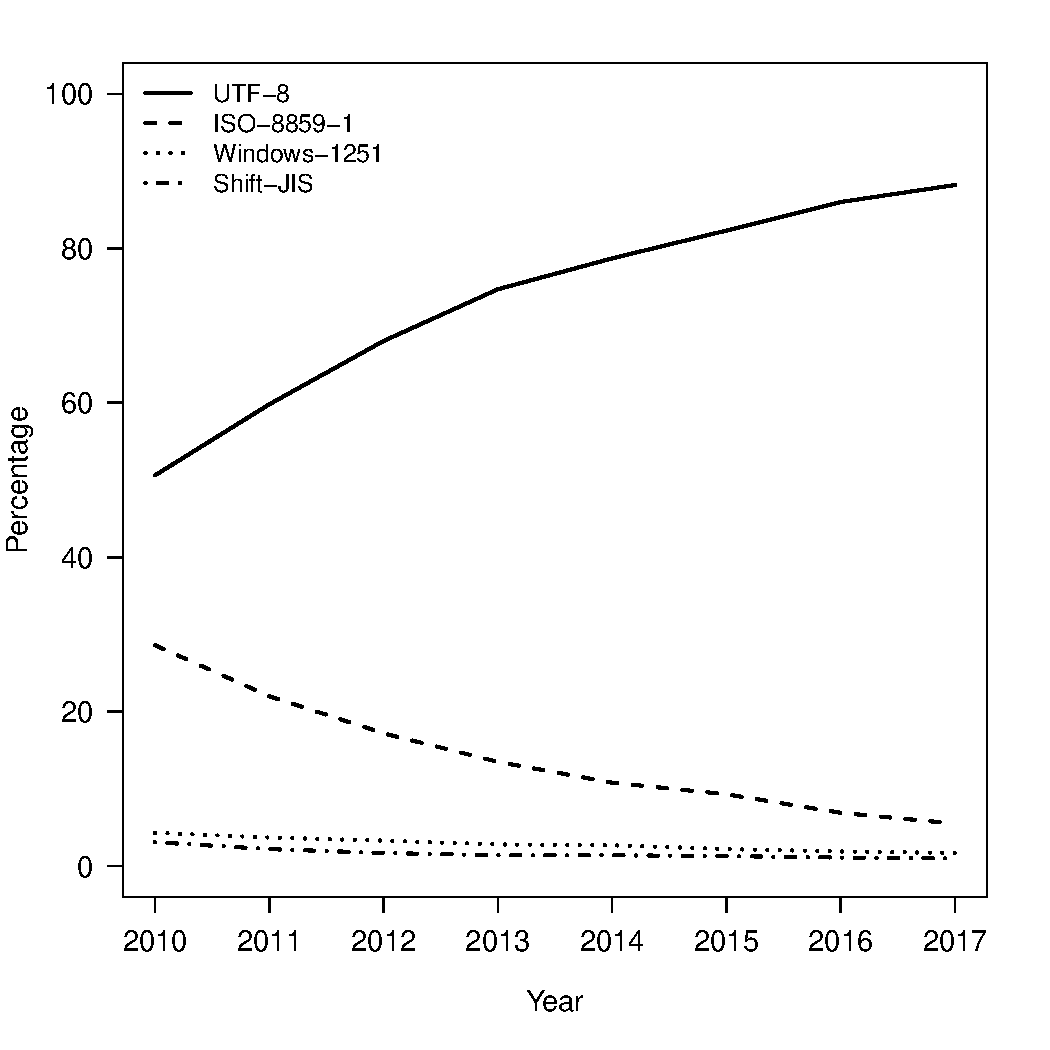
\includegraphics[width=0.7\textwidth]{fig/encoding_use.pdf}
\caption{Percentages of encoding standards used on the web \citep{w3techs2017}.}
\label{fig:encoding}
\end{figure}

The different data types within a file are to be formatted according to
commonly used standards where possible. In particular, data in validation
reports are encoded as stated in Table~\ref{tab:dataformat}.
\begin{center}
\captionof{table}{Format of data types in validation reports.}
\begin{tabular}{|lp{0.92\textwidth}|}
\hline
1&Numbers are encoded in a valid decimal ISO/IEC/IEEE 60559:2011 (IEEE 754) format
\citep{ieee:2008}. \\
2&Date-time data shall be denoted in ISO 8601 format \code{YYMMDDTHHmmss+HHMM} \citep{iso2004data}. \\
\hline
\end{tabular}
\label{tab:dataformat}
\end{center}

%%%%%%%%%%%%%%%%%%%%%%%%%%%%%%%%%%%%%%%%%%%%%%%%%%%%%%%%%%%%%%%%%%%%%%%%%%%%%%%
\clearpage{}
\subsection{JSON messages}
\label{sect:jsonmessage}
To implement the basic and extended validation report we devise a simple object
model allowing for reuse of some components. Recall that the basic results are
identified as a \emph{confrontation} (Definition~\ref{def:confrontation}) and
aggregates are identified as a \emph{aggregation}
(Definition~\ref{def:aggregation}).
We therefore define the following objects.
\begin{align}
\label{eq:confrontation}
\textsf{confrontation} &: 
  \langle\textsf{event}, \textsf{rule}, \textsf{data}, \textsf{value}\rangle\\
\textsf{aggregation}   &:
\langle\textsf{aggregator}, \textsf{nodeset},\textsf{value}\rangle
\end{align}
The mandatory and optional subcomponents of these objects have been discussed
in Sections~\ref{sect:idevent}--\ref{sect:valres} and \ref{sect:aggregators}--\ref{sect:nodesets}.

JSON schemas that define a transmission format for these objects are given in
Listings~\ref{lst:confrontation} and \ref{lst:aggregation}, on pages
\pageref{lst:confrontation} and \pageref{lst:aggregation} of the next section
respectively. Listing~\ref{lst:exampleconfrontation} shows an example
confrontation JSON message, conforming to this standard. Note that this is not
yet a full validation report since this would allow for multiple confrontations
to be stored.  In this example, a validation event was executed using R version
3.4.0 on 18 May 2017 at 10:50:55, in the UTC+2 timezone (this is CEST,
summertime).  The rule is stated using syntax accepted by R package
\code{validate} version 0.1.7, and the expression is \code{income >=  0}.
Failure to pass this rule indicates an error, and there is also a short
description. The data under scrutiny is coded in a length 4 array using the
$U\tau uX$ model for data identification.  In this case the household income of
household number \code{"8237193679"}, as collected during the Household survey
of 2017 amongst Dutch inhabitants was checked. The result is \code{1}, meaning
that the test is passed.
%
\begin{lstlisting}[
  frame=single
  , float=h
  , caption=An example JSON confrontation message
  , label=lst:exampleconfrontation]
{
  "event": {
    "time": "20170518T105055+02",
    "actor": "R 3.4.0",
    "agent": null,
    "trigger": null
  },
  "rule": {
    "language": "R pkg validate 0.1.7",
    "expression": "income >= 0",
    "severity": "error",
    "description": "total income must be non-negative"
  },
  "data": [
    "Dutch inhabitants",
    "Household survey 2017",
    "8237193679",
    "Household Income"
  ],
  "value": "1"
}
\end{lstlisting}
\begin{lstlisting}[
  frame=single
  , linewidth=1.1\textwidth
  , float=h
  , caption=An example JSON aggregation message
  , label=lst:exampleaggregation
  ]
{
  "aggregator": {
    "language": "R 3.4.0",
    "expression": "mean(x,na.rm=TRUE)",
    "description": "Fraction of non-NA events passing."
  },
  "nodeset": {
    "keys": [
      "x0coffee",
      "x0beefed"
    ],
    "description": "All confrontations."
  },
  "value": "0.5"
}
\end{lstlisting}

An example aggregation message is shown in
Listing~\ref{lst:exampleaggregation}.  This partial message conveys an
aggregate, computed using R 3.4.0 with the expression \code{mean(x,
na.rm=TRUE)}. According to the description this results in the fraction of
passes, computed over the values that actually resulted in a value (not \na{}).
The nodes over which this fraction is computed are identified with hexadecimal
keys \code{0xcoffee} and \code{0xbeefed}, which according to the description
corresponds to all confrontations in the complete message.
%


Now that the basic information components have been defined, we can define the
basic and extended validation report. A JSON message containing a validation
report is just an array of confrontations. The JSON schema is given in
Listing~\ref{lst:basic}.

The extended validation report represents a directed acyclic graph.  Each node
in this graph is represented as a key-value pair where the payload can either
be a confrontation, corresponding to the result of a single validation event,
or an aggregate.  Symbolically (using `$|$' to indicate `or'):
\begin{align}
\label{eq:node}
\textsf{node} &: \langle \textsf{key},\textsf{value}\rangle\textrm{, where }
\textsf{value} : \langle \textsf{confrontation} | \textsf{aggregation}\rangle.
\end{align}


\clearpage{}
%%%%%%%%%%%%%%%%%%%%%%%%%%%%%%%%%%%%%%%%%%%%%%%%%%%%%%%%%%%%%%%%%%%%%%%%%%%%%%%
\subsection{JSON Schemas}
In this subsection the JSON schemas defining the basic and extended
validation reports and their components are listed as a reference.

The full code can also be found at github:
\begin{center}
\href{https://github.com/data-cleaning/ValidatReport}{https://github.com/data-cleaning/ValidatReport}
\end{center}
%
\lstinputlisting[frame=single
  , float=h,caption=JSON schema for a confrontation object.
  , label=lst:confrontation]{../json/confrontation.json}
%
%
\lstinputlisting[frame=single
  , float=h
  , linewidth=1.1\textwidth
  , caption=JSON schema for an aggregation object..
  , label=lst:aggregation]{../json/aggregation.json}
%

%
\lstinputlisting[frame=single
  , float=h
  , caption=JSON schema for basic validation report.
  , label=lst:basic]{../json/basic_validation_report.json}
%




%
\lstinputlisting[frame=single
  , float=h
  , caption=JSON schema for extended validation report.
  , label=lst:extended]{../json/extended_validation_report.json}
%







\clearpage{}
\section{Examples}
In this Section we work out a few examples based on validation reports that are 
currently implemented in several statistical institutes. We are grateful to the
organisations that provided the examples to the ESSnet project.

\lstinputlisting[frame=single
  , linewidth=1.1\textwidth
  , showstringspaces=FALSE
  , caption=Part of an extended report based on an example from the Swedish
    Triton system.
  , label=lst:swedish]{../examples/ex-sweden.json}

\newpage
\lstinputlisting[frame=single
  , linewidth=1.1\textwidth
  , showstringspaces=FALSE
  , caption=Part of an extended report based on the assessment of VTL 1.1 - 
    Questionnaire for NAPS statistics (January 2017).
  , label=lst:vtl]{../examples/ex-assessment.json}




\clearpage{}
\bibliography{report}
\end{document}
